\documentclass[a4paper,14pt]{extarticle}

\usepackage{cmap}
\usepackage[T2A]{fontenc}
\usepackage[utf8x]{inputenc}
\usepackage[english, russian]{babel}

\usepackage{misccorr} % в заголовках появляется точка, но при ссылке на них ее нет
\usepackage{amssymb,amsfonts,amsmath,amsthm}  
\usepackage{indentfirst}
\usepackage[usenames,dvipsnames]{color} 
\usepackage[unicode,hidelinks]{hyperref}
% \hypersetup{%
%     pdfborder = {0 0 0}
% }
\usepackage{physics}
\DeclareMathOperator{\Div}{div}
\DeclareMathOperator{\Rot}{rot}
\DeclareMathOperator{\Grad}{grad}
\DeclareMathOperator{\const}{const}
\usepackage{makecell,multirow} 
\usepackage{ulem}
\usepackage{graphicx,wrapfig}
\graphicspath{{img/}}
\usepackage{geometry}
\geometry{left=1cm,right=1cm,top=1cm,bottom=2cm,bindingoffset=0cm}
\usepackage{fancyhdr,float} 
\renewcommand{\phi}{\varphi}
\renewcommand{\epsilon}{\varepsilon}
\renewcommand{\kappa}{\varkappa}


\newcommand{\ticket}[1] {
\newpage
\hypertarget{num#1}{}
\begin{center}
	\textbf{Вопрос минимума №#1 }
\end{center}
}


\linespread{1.05} 
\frenchspacing 
\begin{document}
	\begin{center}
		\Large \textbf{Программа минимум по электродинамике}
	\end{center}
		\textit{Записать формулы и построить графики (без вывода), объяснить используемые в них обозначения: дать требуемые определения}
	\begin{enumerate}
		\item 
		\hyperlink{num1}{Запись функции, определяющей зависимость полей и векторных потенциалов гармонической плоской волны в линии передачи от времени $t$ и продольной координаты $z$. Понятия частоты, временного периода, продольного волнового числа, длины волны, фазовой и групповой скорости.}
%		\hyperref[num1]{Запись функции, определяющей зависимость полей и векторных потенциалов гармонической плоской волны в линии передачи от времени $t$ и продольной координаты $z$. Понятия частоты, временного периода, продольного волнового числа, длины волны, фазовой и групповой скорости.}
		
		\item 
		\hyperlink{num2}{Волновое уравнение для векторного потенциала в отсутствие источников при произвольной и гармонической зависимости от времени. Дифференциальное уравнение для функций поперечных координат $\phi^{(e)}$ и $\phi^{(m)}$. Понятие поперечного волнового числа.}
		\item 
		\hyperlink{num3}{Понятие о TE, ТМ и ТЕМ волнах. Импедансная связь поперечных компонент полей. Определение поперечного волнового импеданса.}
		\item
		\hyperlink{num4}{Граничные условия для полей и функций  $\phi^{(e)}$ и $\phi^{(m)}$ в линиях передачи с идеально 
		проводящими границами. Математическая формулировка задачи отыскания собственных волн различных типов в идеальной линии.}
		\item 
		\hyperlink{num5}{Дисперсионное уравнение для волн в идеальных линиях. Понятие критической частоты и критической длины волны. Графики зависимости полей от продольной координаты в различные моменты времени при частотах, больших или меньших критической. Зависимости длины волны, фазовой и групповой скорости в линии передачи от частоты.}
		\item
		\hyperlink{num6}{В каких линиях могут существовать главные (TEM) волны? Поля TEM волны в	коаксиальной линии.}
		\item 
		\hyperlink{num7}{Спектр поперечных волновых чисел прямоугольного волновода. Низшая мода (поперечное волновое число, графики поля, картина силовых линий). Низшая мода круглого волновода (поперечное волновое число, картина силовых линий).}
		\item
		\hyperlink{num8}{Причины затухания волн в линиях передачи. Описание затухания, обусловленного потерями энергии в заполняющей среде. Графики зависимости поля в линии передачи с потерями от продольной координаты в различные моменты времени.}
		\item
		\hyperlink{num9}{Описание главных волн в линиях передачи в терминах тока и напряжения: определения величин тока и напряжения, погонной емкости и индуктивности, \underline{определения} волнового сопротивления, импеданса нагрузки, импеданса в любом сечении линии с произвольной нагрузкой на конце.}
		\item 
		\hyperlink{num10}{Коэффициент отражения волны от нагрузки на конце линии. Понятие согласования линии с нагрузкой.}
		\item 
		\hyperlink{num11}{Спектр собственных частот идеального прямоугольного резонатора. Низшая мода прямоугольного резонатора (собственная частота, структура поля).}
		\item 
		\hyperlink{num12}{Причины затухания колебаний в реальных резонаторах. Описание затухания, обусловленного потерями энергии в заполняющей среде. График зависимости поля собственного колебания в реальном резонаторе от времени}
		\item 
		\hyperlink{num13}{Представление полей, создаваемых в волноводе заданными сторонними токами, в виде суперпозиции полей собственных мод (общий вид формул возбуждения волноводов)}
		\item 
		\hyperlink{num14}{Представление полей, создаваемых в резонаторе заданными сторонними токами, в виде суперпозиции полей собственных колебаний (общий вид формул возбуждения резонатора). Резонансные свойства полей.}
		\item 
		\hyperlink{num15}{Способы возбуждения волноводов и резонаторов при помощи штыря и петли.}
		\item 
		\hyperlink{num16}{Определения дифференциального и полного сечений рассеяния тела. Выражение для амплитуды поля и плотности потока энергии рассеянной волны в дальней зоне через дифференциальное сечение рассеяния.}
		\item 
		\hyperlink{num17}{Условие применимости приближения геометрической оптики в задачах дифракции.}
		
	\end{enumerate}
	
	Задачи № 10.1 (а), 10.2, 10.4(а,б), 10.5(а,б), 10.7, 10.8, 10.16, 10.18(6), 10.19, 10.22, 10.23, 10.31(а,б), 10.33 (резонатор без плазмы), 10.35(a), 10.36, 10.38, 10.48, 11.1(1,2,3)
	(В.Б. Гильденбург, М.А. Миллер, Сборник задач по электродинамике, 2001 г.).
	\ticket{1}
	Для плоской гармонической волны (TEM) функция, определяющая зависимость полей, задается следующим образом 
	
	$$\vec{A}^e = \phi^e(\vec{r}_\perp)e^{-ihz}\vec{z}_0$$
	Где $\vec{A}^e$ -- векторный потенциал поля, а $\phi^e(\vec{r}_\perp)$ называется поперечной волновой функцией. Поля $\vec{E}$ и $\vec{H}$ определяются следующим образом
	$$\vec{H}=\frac{1}{\mu} rot\vec{A}^e $$
	$$\vec{E}=-\frac{1}{c} \pdv{\vec{A}^e}{t}-\nabla{\phi} $$
	Где $\phi$ -- скалярный потенциал поля. 
	Используя условие калибровки Лоренца
	$$div\vec{A}^e+\frac{\epsilon\mu}{c}i\omega\phi=0$$
	Получим выражения для нахождения полей $\vec{E}$ и $\vec{H}$ в случае гармонической волны:
	$$\vec{H}=\frac{1}{\mu} rot\vec{A}^e $$
	$$\vec{E}=\frac{1}{i k_0\epsilon\mu}(\nabla div + k^2)\vec{A}^e $$
	$$k_0=\frac{\omega}{c}, \quad k=\frac{\omega}{c}\sqrt{\epsilon\mu}$$
	
	Понятие частоты $\omega$ -- равна количеству повторений или возникновения событий (процессов) в единицу времени.
	
	Понятие временного периода $T = \frac{2\pi}{\omega}$ -- время, за которое совершается полное колебание.
	
	Понятие продольного волнового числа $h=\frac{2\pi}{\lambda}$ -- волновым числом  называется быстрота роста фазы волны по пространственной продольной координате.
	
	Понятие длины волны $\lambda$ -- пространственный период колебаний. Расстояние между двумя ближайшими друг к другу точками в пространстве, в которых колебания происходят в одинаковой фазе.
	
	Понятие фазовой $v_{\text{ф}}$ и групповой скорости $v_{\text{гр}}$. Фазовая скорость -- скорость перемещения поверхности постоянной фазы. Групповая скорость -- скорость перемещения квазимонохроматического пакета.
	$$v_{\text{ф}}=\frac{\omega}{h}, \quad v_{\text{гр}}=\pdv{\omega}{h} \Bigl|_{\omega=\omega_0}$$
	Где $\omega_0$ -- несущая частота группового пакета.
	
	\ticket{2}
	Волновое уравнение для векторного потенциала в случае произвольной зависимости от времени и отсутствия сторонних источников
	$$\Delta\vec{A} -\frac{\epsilon\mu}{c^2}\pdv[2]{\vec{A}}{t}=0$$ 
	Волновое уравнение для векторного потенциала в случае гармонической зависимости от времени и отсутствия сторонних источников
	$$\Delta\vec{A} + k^2 \vec{A}=0$$
	$$\pdv{}{t} \to i\omega, \quad k^2=\frac{\omega^2}{c^2}\epsilon\mu$$
	Дифференциальное уравнение для функций поперечных координат $\phi^{(e)}$ и $\phi^{(m)}$. Понятие поперечного волнового числа.
	$$\vec{A}^e = \phi^e(\vec{r}_\perp)e^{-ihz}\vec{z}_0$$
	$$\Delta = \pdv[2]{}{x}+\pdv[2]{}{y}+\pdv[2]{}{z}=\Delta_\perp+\pdv[2]{}{z}$$ -- для декартовой системы координат.
	$$\Delta A_z^e + k^2 A_z^e=\Delta_\perp\phi^e + (k^2-h^2)\phi^e=0$$
	Тогда дифференциальное уравнение для функций поперечных координат $\phi^{(e)}$ и $\phi^{(m)}$  выглядит следующим образом
	$$\Delta_\perp\phi^{(e,m)} + \kappa^2\phi^{(e,m)}=0$$
	Где $\kappa$ -- поперечное волновое число. 	
	Если функции $\phi^{(e)}$ и $\phi^{(m)}$ удовлетворяют двумерному уравнению Гельмгольца, то поля удовлетворяют уравнению Максвелла.
	
	\ticket{3}
	Используем выражения для полей через векторный потенциал
	$$\vec{H}=\frac{1}{\mu} rot\vec{A}^e $$
	$$\vec{E}=\frac{1}{k_0\epsilon\mu}(\nabla div + k^2)\vec{A}^e $$
	Вычислим $\nabla div \vec{A}^e$ и $rot \vec{A}^e$ при условии $\vec{A}^e = \phi^e(\vec{r}_\perp)e^{-ihz}\vec{z}_0$
	$$div \vec{A}^e = -ih\phi^e(\vec{r}_\perp)e^{-ihz}$$
	$$\nabla div \vec{A}^e = (-h^2\phi^e\vec{z}_0-ih\nabla_\perp\phi^e)e^{-ihz}$$
	$$rot \vec{A}^e = [\nabla A^e_z,\vec{z}_0] = [\nabla_\perp\phi^e,\vec{z}_0]e^{-ihz}$$
	Тогда получим следующие выражения для комплексных амплитуд полей TM волны 
	\begin{displaymath}
	e^{-ihz}\cdot
	\begin{cases}
	$$\displaystyle E_z = \frac{\kappa^2}{k_0\epsilon\mu}\phi^e(\vec{r}_\perp)$$ \\
	$$\displaystyle\vec{E}_\perp = -\frac{h}{k_0\epsilon\mu}\nabla_\perp\phi^e(\vec{r}_\perp)$$ \\
	$$\displaystyle\vec{H}_\perp = \frac{1}{\mu}[\nabla_\perp\phi^e(\vec{r}_\perp,\vec{z}_0)]$$ \\
	$$\displaystyle H_z = 0$$
	\end{cases}
	\end{displaymath}

	TM - поперечная магнитная волна. Магнитное поле чисто поперечно пути распространения, но поле $\vec{E}=\vec{E}_\parallel+\vec{E}_\perp$ имеет продольную и поперечную составляющую.
	
	Уравнения Максвелла симметричны относительно полей, но мы получили неравноправные выражения для векторов. Это объясняется тем, что мы нашли одно из решений. Воспользовавшись принципом двойственности $\vec{E}\to\vec{H}$, $\vec{H}\to -\vec{E}$, можно получить выражения  для комплексных амплитуд полей TE волны. 
	\begin{displaymath}
	e^{-ihz}\cdot
	\begin{cases}
	$$\displaystyle H_z = \frac{\kappa^2}{k_0\epsilon\mu}\phi^e(\vec{r}_\perp)$$ \\
	$$\displaystyle\vec{H}_\perp = -\frac{h}{k_0\epsilon\mu}\nabla_\perp\phi^e(\vec{r}_\perp)$$ \\
	$$\displaystyle\vec{E}_\perp = -\frac{1}{\epsilon}[\nabla_\perp\phi^e(\vec{r}_\perp,\vec{z}_0)]$$ \\
	$$\displaystyle E_z = 0$$
	\end{cases}
	\end{displaymath}
	функция $\phi$ не обязана быть такой же, поэтому изменяется верхний индекс на $m$, эта функция также должна удовлетворять уравнению Гельмгольца  
	$$\Delta_\perp\phi^{m} + \kappa^2\phi^{m}=0$$
	Таким образом для системы уравнений Максвелла возможны два решения TM и TE волны. Но есть случай, когда поля чисто поперечны это случай TEM волны.
	Когда $\kappa = 0$, то есть $k=h$, продольные компоненты магнитного и электрического полей отсутствуют это и есть TEM волна.
	\begin{displaymath}
	e^{-ihz}\cdot
	\begin{cases}
	$$\displaystyle H_z = E_z = 0$$ \\
	$$\displaystyle\vec{E}_\perp = -\frac{1}{\epsilon\mu}\nabla_\perp\phi(\vec{r}_\perp)$$ \\
	$$\displaystyle\vec{H}_\perp = \frac{1}{\mu}[\nabla_\perp\phi(\vec{r}_\perp,\vec{z}_0)]$$ 
	\end{cases}
	\end{displaymath}
	$\phi$ -- поперечная волновая функция, удовлетворяющая уравнению $\Delta\phi=0$.
	Из формул выше видно, что поперечные компоненты полей удовлетворяют импедансному соотношению
	$$\vec{E}_\perp = \eta_{\perp\text{в}}[\vec{H}_\perp,\vec{z}_0]$$
	где $\eta_{\perp\text{в}}$ называется поперечным волновым сопротивлением
	$$\eta_{\perp\text{в}}=\sqrt{\frac{\mu}{\epsilon}} \left( \frac{k}{h} \right)^{\pm 1}$$ 
	где <<+>> -- соответствует волне типа TE, а <<-->> -- волне типа TM. Для TEM волны $\displaystyle \eta_{\perp\text{в}}=\sqrt{\frac{\mu}{\epsilon}}$
	
<<<<<<< Updated upstream
	% \ticket{4}
	





\ticket{7}
% 7 вопрос
\paragraph{Спектр поперечных волновых чисел прямоугольного волновода. } Поперечные волновые числа появляются как собственные числа решения уравнения Гельмгольца с граничными условиями прямоугольного волновода. Спектр найденных таким образом собственных чисел описывается формулой
\begin{equation}
	\varkappa^2_{mn} = \qty(\frac{m\pi}{a})^2+
		\qty(\frac{n\pi}{b})^2
\end{equation}
Здесь $m$, $n$ -- индексы моды, $a$, $b$ -- размеры сечения волновода. Для однозначности мы всегда считаем, что $a>b$.

\paragraph{Низшая мода.} По определению, такой модой называется мода с наименьшим поперечным волновым числом. Так как мы предполагали $a>b$, очевидно, наименьшее возможное нетривиальное поперечное волновое число будет при $m=1$, $n=0$:
\begin{equation}
	\varkappa^2_{10} = \frac{\pi^2}{a^2}
\end{equation}
Заметим, что это возможно только для TE-волн, так как решение TM-волн не позволяет занулить $m,n$ одновременно (это приведет к тривиальной поперечной волновой функции). Так что \textit{низшая мода прямоугольного волновода -- TE${}_{10}$}.
\begin{figure}[h!]
	\centering
	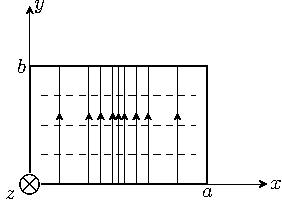
\includegraphics[scale=1.5]{img/lect4_ris8} 
	\caption{Структура полей $\vec{E}$ и $\vec{H}$ моды TE${}_{10}$ ($\vec{H}$ изображено пунктиром)}
	\label{fig:lect4:8}
\end{figure}

\paragraph{Низшая мода круглого волновода .} Она определяется так же, но решение уравнения идет в бесселевых функциях, и поэтому поперечное волновое число имеет другой вид, и низшей модой будет TE${}_{11}$:
\begin{equation}
	\varkappa_{11}=\frac{\mu_{11}}{a},
\end{equation}
где $\mu_{11}$ -- значение аргумента функции Бесселя $J_1$ при   $1$-м нуле своей прозводной. При этом график моды будет похож на график в прямоугольном волноводе: его можно получить чисто геометрически, постепенно сминая границы волновода, делая его более круглым. Говоря более точно, топологически эти моды подобны.
\begin{figure}[H]
	\centering
	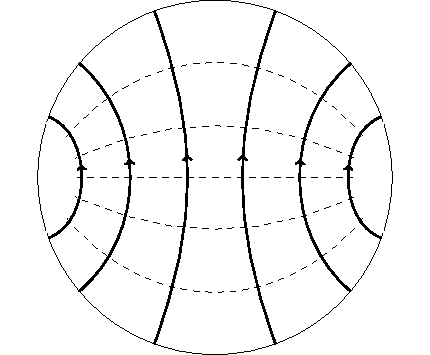
\includegraphics[scale=1.5]{img_lect5/cylindric/TE11.pdf}
	\caption{Структура полей $\vec{E}$ и $\vec{H}$ моды TE${}_{11}$ круглого волновода ($\vec{H}$ изображено пунктиром)}
	\label{fig:lect4:8}
\end{figure}




\ticket{8}
% \phantomsection\addcontentsline{toc}{subsection}{Причины затухания волн в линиях передачи. Описание затухания, обусловленного потерями энергии в заполняющей среде. Графики зависимости поля в линии передачи с потерями от продольной координаты в различные моменты времени.}%
\paragraph{Причины затухания волн в линиях передачи.} В реальных линиях передачи волна распространяется с затуханием за счет \textit{двух} причин: \textit{потери в заполняющей волновод среде} и \textit{потери в стенках волновода}. Мы их учитываем по-отдельности: решаем задачу о потерях в среде, считая стенки $\sigma=\infty$, и наоборот.

\paragraph{Описание затухания, обусловленного потерями энергии в заполняющей среде. } Чтобы учесть потери в среде, подставим комплексную диэлектрическую проницаемость в дисперсионное уравнение:
\begin{equation}
	\varepsilon_k = 
		\varepsilon'-i\frac{4\pi\sigma}{\omega} 
	\quad \to \quad
	h^2 = \frac{\omega^2}{c^2}\varepsilon \mu - \kappa
\end{equation}
Расчеты проводятся при $\mu=1$. Волновое число становится комплесным $h=h'+ih''$, и в случае малых потерь можно найти  $h''$, которое определяет затухание. Для частот, далеких от критической, 
\begin{equation}
	h'' = \frac{\varepsilon'' k_0^2}{2h'}, \qq{где} 
	h' = \sqrt{\frac{\omega^2}{c^2}\varepsilon'-\kappa^2}
\end{equation}
При $\omega>\omega_\text{cr}$ амплитуда волны уменьшается в $e$ раз на расстоянии $L=\qty(h'')^{-1}$. Нетрудно нарисовать графики: это будет сдвигающаяся волна с огибающей в виде спадающей экспоненты.

\paragraph{Графики зависимости поля в линии передачи с потерями от продольной координаты в различные моменты времени.}
Здесь синим цветом показан график в следущий момент времени, желтым - в предыдущий, зеленым - огибающая (экспонента).
\begin{figure}[H]
	\centering 
	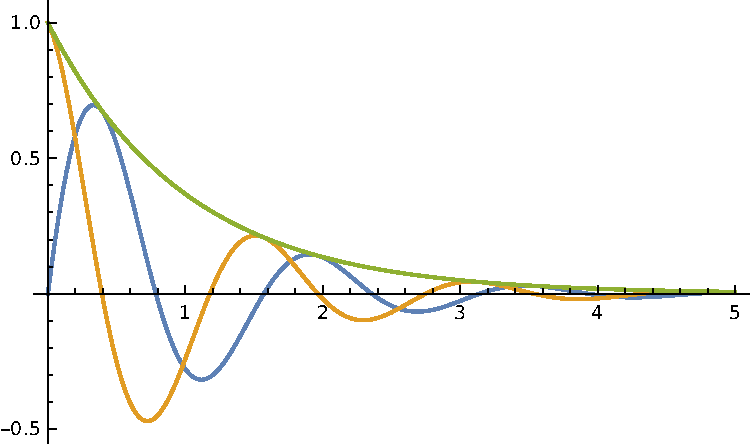
\includegraphics[scale=1]{img2/volna.pdf}
	\caption{Затухание поля в линии передачи}
	\label{fig:lect4:8}
\end{figure}


\ticket{9}
\paragraph{Описание главных волн в линиях передачи в терминах тока и напряжения. } В системе проводников, когда их количество больше или равно двум, могут распространяться главные (ТЕМ) волны. Именно их, в случае двухпроводной линии, можно описать с помощью телеграфных уравнений:
\begin{equation}
	\left\{\begin{aligned}
		\pdv{I}{z} = -C\pdv{V}{t}\\
		\pdv{V}{z} = -\frac{L}{c^2} \pdv{I}{t}
	\end{aligned}\right.
\end{equation}
Они были написаны раньше, чем уравнения Максвелла. Они не дают информации о поле во всем пространстве, а оперируют только интегральными характеристиками: током $V(z,t)$ и напряжением $I(z,t)$\footnote{Продифференцировав второе уравнение по $z$ и первое по $t$, и подставив первое во второе, мы получим волновое уравнение.}.
Здесь введен ряд понятий, которые надо раскрыть подробнее.

\paragraph{Погонные емкость $C$, индуктивность $L$.} Они вводятся как емкость (индуктивность) на единицу длины, или, выражаясь физически более верно, это отношение емкости (индуктивности) бесконечно малого отрезка двухпроводной линии к её длине. Так же вводится \textit{погонный заряд $Q$}.

\paragraph{Напряжение. } По определению, напряжение в двухпроводной линии, в которой распространяется главная волна, будет интеграл
\begin{equation}
	V(z) = \int\limits_{(1)}^{(2)} E_l\, \dd l,
\end{equation}
где интегрирование ведется в плоскости сечения $z=\const$ от одного провода до другого, и не зависит от формы контура. Такое возможно в случае потенциальных полей: поле же главной волны в поперечном сечении потенциально ($\vec{E}=-\Grad \phi$). Хотя в целом оно не потенциально:
\begin{equation}
	\Rot \vec{E} = \Rot\qty[
		\nabla_\perp \phi(\vec{r}_\perp)\cdot e^{-ihz}
	]
\end{equation}

\paragraph{Ток. } Ток в сечении двухпроводной линии есть отношение количества заряда, проходящего в единицу времени через сечение $z=\const$ одного провода, к единице времени ($I=\dd{Q}/\dd{t}$). 

\paragraph{Волновое сопротивление (характеристический импеданс). } В терминах тока и сопротивления, это есть отношение напряжения бегущей волны к току бегущей волны в одном сечении. Выражение можно получить, подставив $V=V_0\cdot e^{i(\omega t \pm kz)},\, I=I_0\cdot e^{i(\omega t \pm kz)}$ в волновое уравнение:
\begin{equation}
	Z_\text{в}=\qty|\frac{V_\text{бег}(z)}{I_\text{бег}(z)}|=\frac{1}{c}\sqrt\frac{L}{C}
\end{equation}

\paragraph{Импеданс нагрузки. } Он вводится как отношение напряжения на нагрузке к току в нагрузке:
\begin{equation}
	Z_\text{н}=\frac{V_\text{н}}{I_\text{н}}
\end{equation}

\paragraph{Импеданс в произвольном сечении линии. } Он определяется как $Z(z) = V(z)/I(z)$, и с этим тесно связана формула пересчета импеданса, а именно, можно узнать импеданс в любом сечении линии, зная волновой импеданс и импеданс произвольной нагрузки на конце. Тогда, считая положение нагрузки в $z=0$, формула принимает вид
\begin{equation}
	Z(z=-L) = Z_\text{в}\frac{Z_\text{н}+iZ_\text{в}\tg kL}{Z_\text{в} + i Z_\text{н} \tg kL}
\end{equation}




\ticket{10}
\paragraph{Коэффициент отражения волны от нагрузки на конце линии. } Это может быть коэффициент отражения по току или по напряжению. Обычно, когда не упоминается чего, считается, что напряжения. По определению, это
\begin{equation}
	\Gamma = \frac{V_\text{отр}}{V_\text{пад}} = \text{(если посчитать)} = 
	\frac{Z_\text{н}-Z_\text{в}}{Z_\text{н}+Z_\text{в}}
\end{equation}

\paragraph{Понятие согласования линии с нагрузкой. } Линия называется согласованной, если нет отраженной волны: $\Gamma=0$. Для этого нужно, чтобы было $Z_\text{н}=Z_\text{в}$.




\ticket{11}
\paragraph{Спектр собственных частот идеального прямоугольного резонатора.} Его можно найти, если взять прямоугольный волновод и металлизировать сечения нулей электрического поля, удовлетворив граничному условию $E_\tau=0$:
\begin{equation}
	\omega_{mnp} = \frac{\pi c}{\sqrt{\varepsilon \mu}} \sqrt{\frac{m^2}{a^2}+\frac{n^2}{b^2}+\frac{p^2}{L^2}},
\end{equation}
где $a>b$ -- размеры поперечного сечения, $L$ -- длина резонатора.
\paragraph{Низшая мода прямоугольного резонатора. }% собственная частота, структура поля
Если $b<a$, $b<L$, то низшей модой будет TE${}_{101}$:
\begin{equation}
	\omega_{101}=\frac{c}{\sqrt{\varepsilon \mu}}\sqrt{
		\qty(\frac{\pi}{a})^2
		\qty(\frac{\pi}{L})^2
	}
\end{equation}
Надо заметить, что TE/TM здесь условно, так как зависит от выбора осей. Пусть ребро $a$ вдоль $x$, $b$ вдоль $y$, $L$ вдоль $z$.  Структура поля тогда 
\begin{equation}
	\vec{E}=\vec{y}_0 E_0 \sin(\frac{\pi}{a}x)\sin(\frac{\pi}{L}z)e^{i\omega_{101}t}
\end{equation}








\ticket{12}
\paragraph{Причины затухания колебаний в реальных резонаторах.} Как и в случае линии передачи, причин две:
потери в заполняющей среде (комплексная $\varepsilon$) и потери в стенках ($\sigma \ne \infty$).
\paragraph{Затухание за счет потерь в заполнении.} Чтобы его найти, нужно действовать стандартно: представить 
$\varepsilon=\varepsilon'+i \varepsilon''$, аналогично $\mu=\ldots$. Связь частот определяется формулой
\begin{equation}
	\omega=\frac{\omega^{(0)}}{\sqrt{\varepsilon \mu}},
\end{equation}
где $\omega^{(0)}$ -- спектр незаполненного резонатора. Отсюда найдется $\omega''$ ($\omega=\omega'+i \omega''$), и тогда затухание будет происходить как 
\begin{equation}
	E,H  \sim e^{i \omega t} \sim e^{i \omega' t}\cdot e^{-i \omega'' t}
\end{equation}
При $\mu=1$ оказывается, что $\omega''\sim -\varepsilon''$. Это не ошибка, так как $\varepsilon''<0$. %(знак минус -- не ошибка: действительно, $\varepsilon'' = -\frac{4\pi\sigma}{\omega}$)
\paragraph{График собств. колебаний в реальном резонаторе от времени.} Для прямоугольного резонатора можно построить $\mathrm{Re}\, E_x(t)$, это будет синусоида, вписанная в огибающую -- убывающую экспоненту:
\begin{figure}[H]
	\centering
	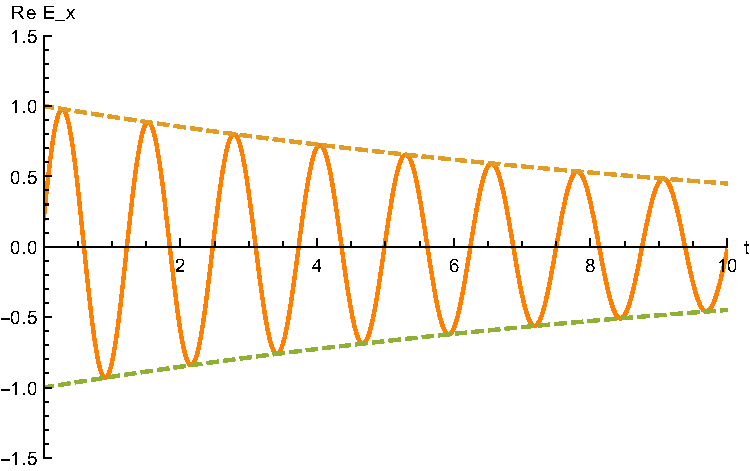
\includegraphics[scale=1]{img2/exp.pdf}
	\caption{Затухание поля в резонаторе со временем}
	\label{fig:figure1}
\end{figure}




\ticket{13}
\paragraph{Представление полей в ЛП как суперпозицию мод.}
\begin{figure}[H]
	\centering
	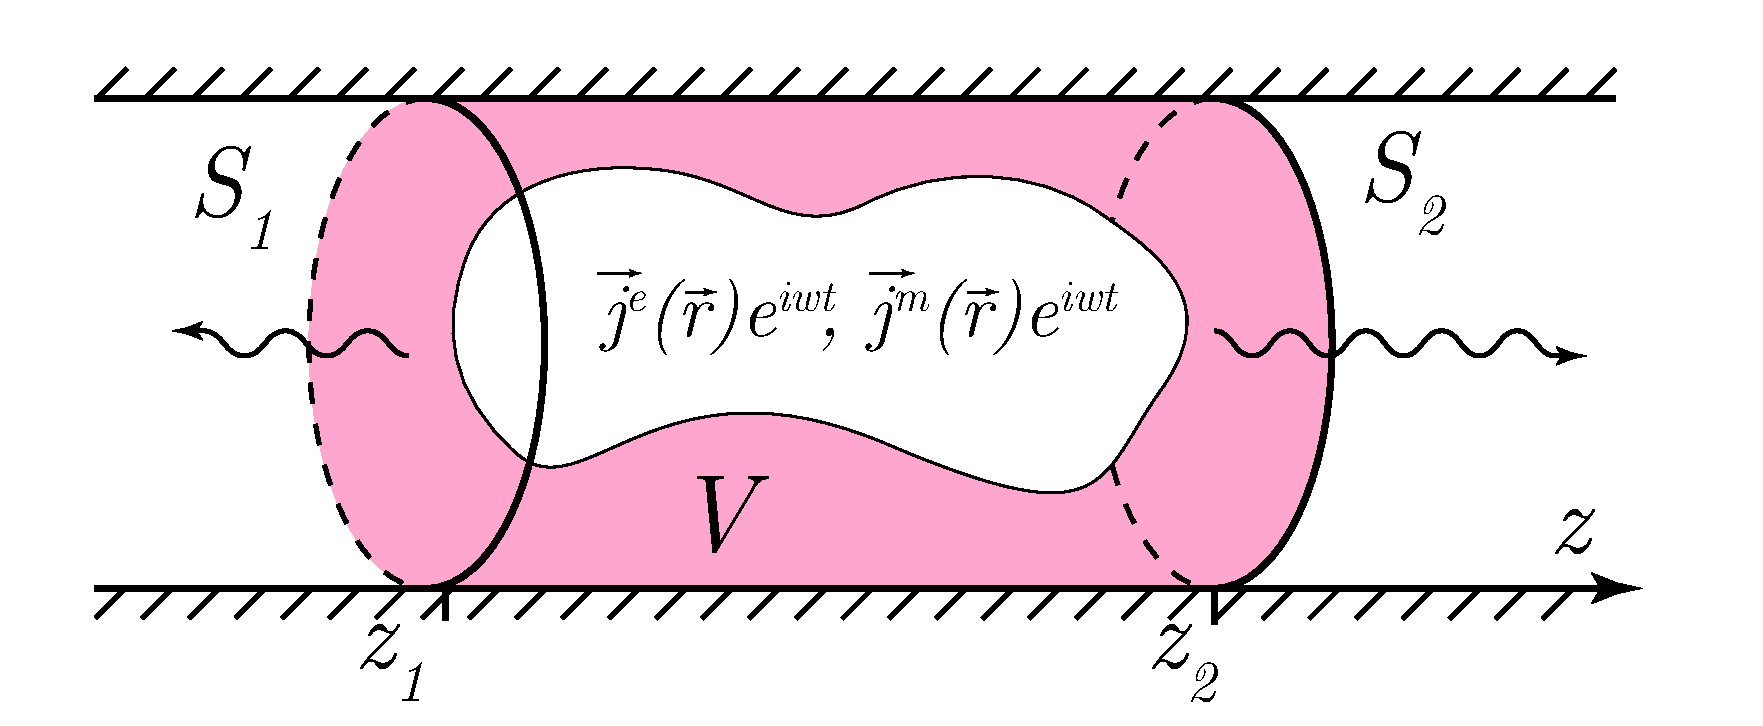
\includegraphics[width=0.6\linewidth]{img/13.pdf}
	\caption{Заданные источники тока в ЛП} 
	\label{fig:figure13}
\end{figure}

Пусть в волноводе в области от $z_1$ до $z_2$ заданы токи $\vec{j}^e$ и $\vec{j}^m$. Тогда поля вне области источников тока можно найти как
суперпозицию собственных мод волновода:
\begin{align*}
	&\vec{E}(z>z_2) = \sum \limits_{p=1}^{\infty}a_p\vec{E}_p\\
	&\vec{E}(z<z_1) = \sum \limits_{p=1}^{\infty}a_{-p}\vec{E}_{-p}	,	
\end{align*}
где $p$ - индекс моды в волноводе. коэффициента $a_p$ и $a_{-p}$ находятся следующим образом:
\begin{align*}
	&a_p = \frac{1}{N_p}\int\limits_V\left[ (\vec{j}^e,\vec{E}_{-p})-(\vec{j}^m,\vec{H}_{-p}) \right]\dd V\\
	&a_{-p} = \frac{1}{N_p}\int\limits_V\left[ (\vec{j}^e,\vec{E}_{p})-(\vec{j}^m,\vec{H}_{p}) \right]\dd V,
\end{align*}
где $N_p$ - это норма моды $p$, $N_p=\pm4\Pi_p$, где $\Pi_p$ - мощность моды типа $p$.


\ticket{15}
\paragraph{Способы возбуждения волноводов и резонаторов при помощи штыря и петли. } Основной идеей является расположение возбуждающего элемента таким образом, чтобы пораждаемое им поле совпадало с полем одной из мод резонатора (или волновода).

\end{document}